\section{Curves in the Plane}
\label{sec:curves}

In this section, we introduce parameterized curves in the plane, define curvature
in this setting, and state another simple version of the Gauss-Bonnet theorem.

\subsection{Parameterized Curves}

A \emph{parameterized curve in the plane} is the image of a map for a closed interval
into the plane
$$\gamma: I\rightarrow \R^2\hspace{1cm} \gamma(t)=(x(t),y(t)).$$ 
One can think of $t$ as time and parameterization indicating a point tracing out the image
of the curve.
If the point never stops moving and there are no cusps in the image and there is a finite number
of transverse crossings then the curve
is said to be \emph{regular}\footnote{Others use the word normal or generic}.
An example is show in \figref{parameterized-curve}.
It takes one number $t$ to specify the position of a point on the curve, so we say our
curves are one dimensional.
Parameterizations also allow us to deal with points where a curve self-intersects, namely 
restrict the parameterization to a local region where the curve does not self-intersect.

A feature of parameterizations is that the velocity of the traversal is included.
For each $t$ we have a tangent vector $$\gamma'(t)=(x'(t),y'(t)).$$
Two different maps can result in the same curve but the speeds that we traverse the curve can be different.
If $\gamma$ is regular then $\gamma'(t)\neq 0$ for all $t$,
and we can normalize the speed of our parameterization
to obtain $$\frac{\gamma(t)}{||\gamma'(t)||},$$ parameterizations with $$\frac{\gamma(t)}{||\gamma'(t)||}=1$$ are said to be parameterized by \emph{arclength}. This means $t$ represents 
the distance traveled along the curve. Unless otherwise specified, we assume our parameterizations are parameterized by arclength.

The velocity vector is $\gamma'(t)=(x'(t),y'(t))$, and the speed is the magnitude of the velocity
$$||\gamma'(t)||=\sqrt{(x'(t)^2)+(y'(t))^2}.$$
Let $$ds=||\gamma'(t)||dt.$$ This number represents the infinitesimal amount of distance traveled along the curve when $t$ changes by an infinitesimal amount and is called th \emph{differential} of arclength along the curve.




\begin{figure}[htb]
\centering
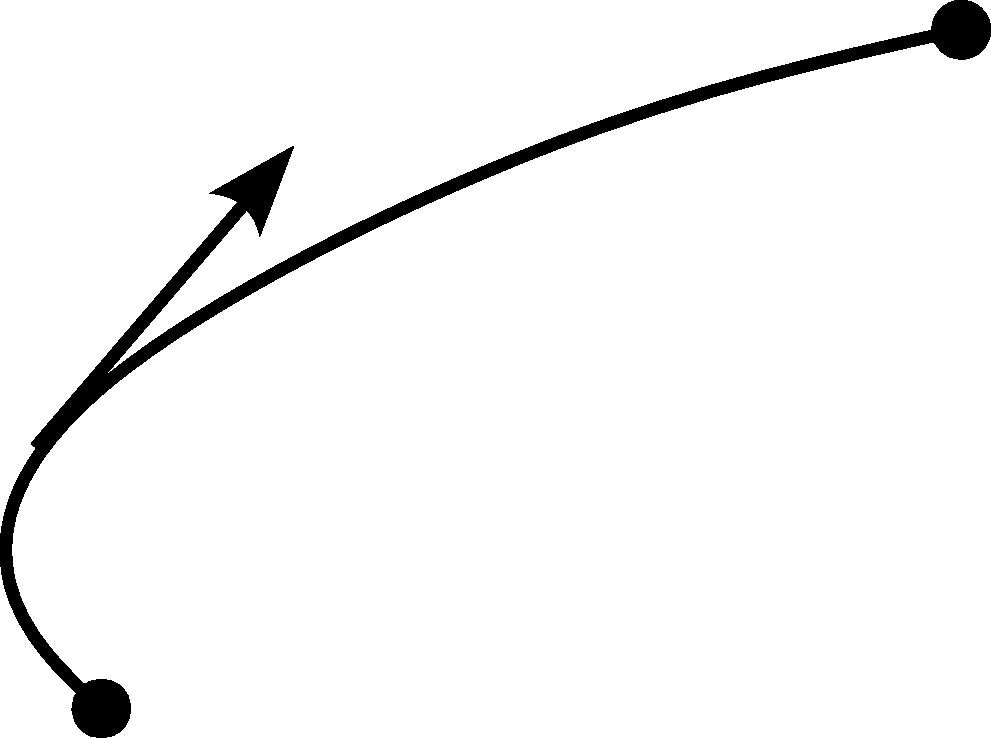
\includegraphics[width=.3\textwidth]{images/parametric}
\caption{The parametric curve $x=t^2-t, y=t-1$ for $0\leq t\leq 3$ and the tangent vector at 
$t=2$.}
\label{fig:parameterized-curve}
\end{figure}


Another example is the unit circle with parameterization given by the map $C:[0,2\pi]\rightarrow \R^2$
$$C(t)=\left(\cos(t),\sin(t)\right).$$ Given a value of $t$ say $\frac{\pi}{2}$ the parameterization
gives a point, namely $(0,1)$. Curves with the property that the initial point is equal to the 
final point are said to be \emph{closed}.
For a parameterized closed curve, instead of the codomain being an interval it is the unit circle $\Sp^1.$

\subsection{Curvature in the Plane}

What do we require of a definition of curvature for a one dimensional curve
in the plane? We would like a number the represents how 
different a curve is from a straight line, so, 
a straight line should have zero curvature.
Ideally,  the unit circle would  have
curvature one. Moreover,
 large circles should have less curvature than smaller circles.
Ideally, definition should also differentiate between
curving to the left and curving to the right.


For any point on a smooth one dimensional curve in the plane,
we can approximate the curve with a circle.
The best approximating circle is called the  \EMPH{osculating circle}.
A natural definition of the \EMPH{curvature} is the inverse of the radius of the osculating
 circle $\kappa=\frac{1}{r}$.
See \figref{osculating-circle} for an example.
The osculating circle meets the requirements for a definition of curvature as long
as we allow the straight line to have an osculating circle with infinite radius.
We determine the sign of the curvature by which side of the curve the osculating circle is on.
However, computing the radius of an osculating circle is somewhat cumbersome.

\begin{figure}[htb]
	\centering
	
\includegraphics[width=.3\textwidth]{curvature/osculating}
	\caption{A curve with two osculating circles. The curvature at these points
	have opposite sign.}
	\label{fig:osculating-circle}
\end{figure}

The circle of radius $r$ in the plane can be parameterized by
$$c(t)=(r\cos(t),r\sin(t))$$
 for $t\in [0,2\pi].$
If a curve is regular, another interpretation of curvature 
is the rate of change
of the angle between the curve and its tangent vector. 
We do not want this
rate to depend on how fast we are traversing the curve and we parameterize by arc length,  in this case, the arc length parameterization
of the circle with radius $r$ is $$C(t)=\left(r\cos\left(\frac{t}{r}\right),r\sin\left(\frac{t}{r}\right)\right).$$

The rate of change of the angle between a curve and its unit tangent vector $T$, is the magnitude
of the derivative of $T$, see \figref{smooth-tangent}. Curvature is then
\begin{equation} \label{eqn:kappa}
\kappa= \pm | T'(t)|.
\end{equation}
where $t$ is arc length.  


For the circle of radius $r$ we have,
$$T(t)=\left(-\sin\left(\frac{t}{r}\right),\cos\left(\frac{t}{r}\right)\right)$$
and 
$$|T'(t)|=\left|\frac{1}{r}\left(-\cos\left(\frac{t}{r}\right),-\sin\left(\frac{t}{r}\right)\right)\right|$$
so
$$\kappa(t)=\frac{1}{r}.$$
We see that,  at least in this case, our definition of curvature in \eqnref{kappa} agrees with the
osculating circle definition. 
For a plane curve $\gamma(t)$ we can summarize above computation as
\begin{equation} \label{eqn:kappa1}
\kappa(t)=\frac{|\gamma'(t)\times \gamma''(t)|}{|\gamma'(t)|^3}.
\end{equation}

What about discrete curves in the plane? A discrete curve is a sequence of connected
line segments. Where two
segments meet there is a corner. The curvature of a point in the interior of a segment
is zero. But what about the corners? Is there a well defined osculating circle? The tangent
vector is not defined!
Consider the exterior angle formed by extending one of the segments, as in \figref{discrete-plane}. 
If the segments are colinear, then the exterior angle is zero. If the interior angle
is smaller, then the curvature is greater as desired.




\begin{figure}[htb]
    \captionsetup[subfigure]{justification=centering}
    \centering
    \begin{subfigure}[b]{0.35\textwidth}
        
\includegraphics[width=\textwidth]{background/interior-angles-triangles}
       \subcaption{}\label{fig:smooth-tangent}
    \end{subfigure}
        \hspace{1cm}
        \begin{subfigure}[b]{0.35\textwidth}
        
\includegraphics[width=\textwidth]{background/discrete-plane}
        \subcaption{}\label{fig:discrete-plane}
        \end{subfigure}
    \caption{(\subref{fig:smooth-tangent}) The tangent vector of a curve in the plane at a point.
        (\subref{fig:discrete-plane}) The exterior angle on a discrete curve in the plane.
    }
    \label{fig:osculating-sphere}
\end{figure}


What about curves in $\R^3$? Now, a curve has more `wiggle room' in that it
 can `twist' vertically out of the plane.
This additional freedom is called torsion.
Let $$\gamma(t)=(x(t),y(t),z(t))$$ be a smooth curve in $\R^3$.
Again, we parameterize by arc length so $|\gamma'(t)|^2=1,$ and the chain rule implies, $\gamma'\cdot \gamma''=0$.
So, $\gamma'$ and $\gamma''$ are orthogonal.
Thus, the
vector $\gamma''=N$ is normal to the $\gamma$. 
By taking the cross product of $N$ and $T$ we obtain a vector $B$ called
the binormal vector.
The vectors $T,N$ and $B$ form the \EMPH{Fernet frame} of $\gamma$ a $p.$


The rate of change of the tangent vector is the curvature and the rate of change in
the binormal is the torsion. If the curve is a straight line for part of the parameterization,
then the Fernet frame is not well defined. We leave it to the reader to think about how to handle
this case.

\subsection{Rotation Number}


Intuitively, the \emph{rotation number} $w(\gamma)$ of a regular closed planar curve is the number
of complete turns the tangent vector makes traversing the curve once.
The winding number $wind(\gamma,p)$ with respect to a point $p$ is the number of times a person standing on $p$ would have to spin around if they held onto a string as the other end point traversed the curve.


A arclength parameterized closed curve is a map $\gamma:\Sp^1\rightarrow \RR^2,$ differentiating
gives a unit vector. This defines a map called, the tangent Gauss map
$$T:\Sp^1\rightarrow \Sp^1,\hspace{1cm} T(t)=\gamma'(t).$$
The \emph{degree} of this map its turning number.



The turning number gives us a way to define a topological equivalence between curves via the Whitney-Graustein theorem. Before stating the theorem we need a few more definitions.
A map is an \emph{immersion} if the differential is injective at every point.
Let
\[
\gamma_0, \gamma_1 : \Sp^1 \to \R^2
\]
be smooth closed curves in the plane.
A \emph{regular homotopy} from $\gamma_0\rightarrow \gamma_1$ is a smooth map
\[
H : \gamma_0 \times [0,1] \to \gamma_1
\]
such that:
\begin{enumerate}
    \item For each \(t \in [0,1]\), the map
    \[
    H_t :  \gamma_0 \to  \gamma_1,
    \qquad
    H_t(x)=H(x,t),
    \]
    is an immersion.

    \item The endpoints satisfy
    \[
    H_0=\gamma_0
    \qquad\text{and}\qquad
    H_1=\gamma_1.
    \]
\end{enumerate}
Two immersions are said to be \emph{regularly homotopic} if there exists a
regular homotopy between them. Informally, a regular homotopy is a continuous deformation through immersions: self-intersections may appear or disappear, but the curve is never allowed to develop a cusp or stop moving, the derivative may never vanish.

The Whitney-Graustein tells us that two curves are `equivalent'
if they have the same turning number.
\begin{theorem}[Whitney--Graustein]
Let
\[
\gamma_0,\gamma_1 : \Sp^1 \to \mathbb{R}^2
\]
be smooth immersed closed curves. Then \(\gamma_0\) and \(\gamma_1\) are
regularly homotopic if and only if they have the same turning number.
\end{theorem}


Our theme is that total rotation of a geometric frame equals a topological invariant.
The turning number gives a special case of the Gauss-Bonnet Theorem for regular closed
curves in the plane. If we add up the curvature at every point we obtain
the turning number and if for any two curves with the same turning number
have the same total curvature.

\begin{theorem}[Gauss-Bonnet for Curves in the Plane]\label{thm:curves-bonnet}
Let $\gamma$ be a closed regular curve in the plane, then
$$\int_\gamma k ds=2\pi w(\gamma).$$
\end{theorem}
\begin{proof}
Let $\theta(s)$ denote the tangent angle,
then $$\kappa=\frac{d\theta}{ds}$$
and
$$\int_\gamma \kappa ds=\int_0^L\frac{d\theta}{ds}ds=\Delta \theta.$$
One full rotation contributes $2\pi,$
$$\Delta \theta=2\pi w(\gamma)$$
combining gives the theorem.
\end{proof}



\noindent \textbf{Exercises}

\begin{enumerate}

	\item Draw two closed curves that are regularly homotopic. And draw two closed curves that are not regularly homotopic.
	
	 \item Give a parameterization of an ellipse in the plane. Compute the tangent vector and curvature at various points.
 
 \item Given a parameterized curve in the plane, give a formula for the osculating circle at a fixed point.
 
 \item Formulate \thmref{simple-bonnet} in terms of curvature.

\end{enumerate}

